\chapter{Testing Usability and Effectiveness on a Wider Audience}
\label{chap:userstudy}

While the results documented in the previous section suggest that CrashSimulator
is effective at finding environmental bugs, we acknowledge that the evaluation
was conducted by developers with a high degree of expertise in its operation,
namely the people who developed it.  We felt it would be prudent to ensure it
would be equally effective when employed by outside developers.
To investigate this angle,
we conducted a user study
with 12 undergraduate and graduate students with varying experience levels.
This study took place over the course of six sessions
of an Application Security class attended by the study participants.
Each class began with 20
minutes of instruction on aspects of using the tool
and the remaining 70 minutes were used as work time. Students then used
CrashSimulator to find bugs in applications and construct patches to fix
them.  They were also encouraged to spend time outside
of class on these efforts.  They were asked to record their progress
using a provided work log template.  These work logs document the participants
progress toward identifying bugs using CrashSimulator and constructing patches
to fix them.  Each weekly entry listed the applications the participant was
working on and what bugs they had found.

Our goal for this user study was two-fold.  First and foremost,
we wanted to see if the students were able to use it to find bugs,
even with only limited instruction and experience with the tool.
We discuss these results in~\ref{subsec:bugs-by-participants}.
Second, we wanted the students to help us identify usability issues
or flaws within the tool itself.  We summarize what the students found
in~\ref{subsec:crashsim-patches}.  Finally, we share our observations
of how students interacted with the tool and what shortcomings
it revealed in~\ref{subsec:tool-shortcomings}.

\newgeometry{left=2cm}
\begin{figure}[btp]
\centering
\fbox{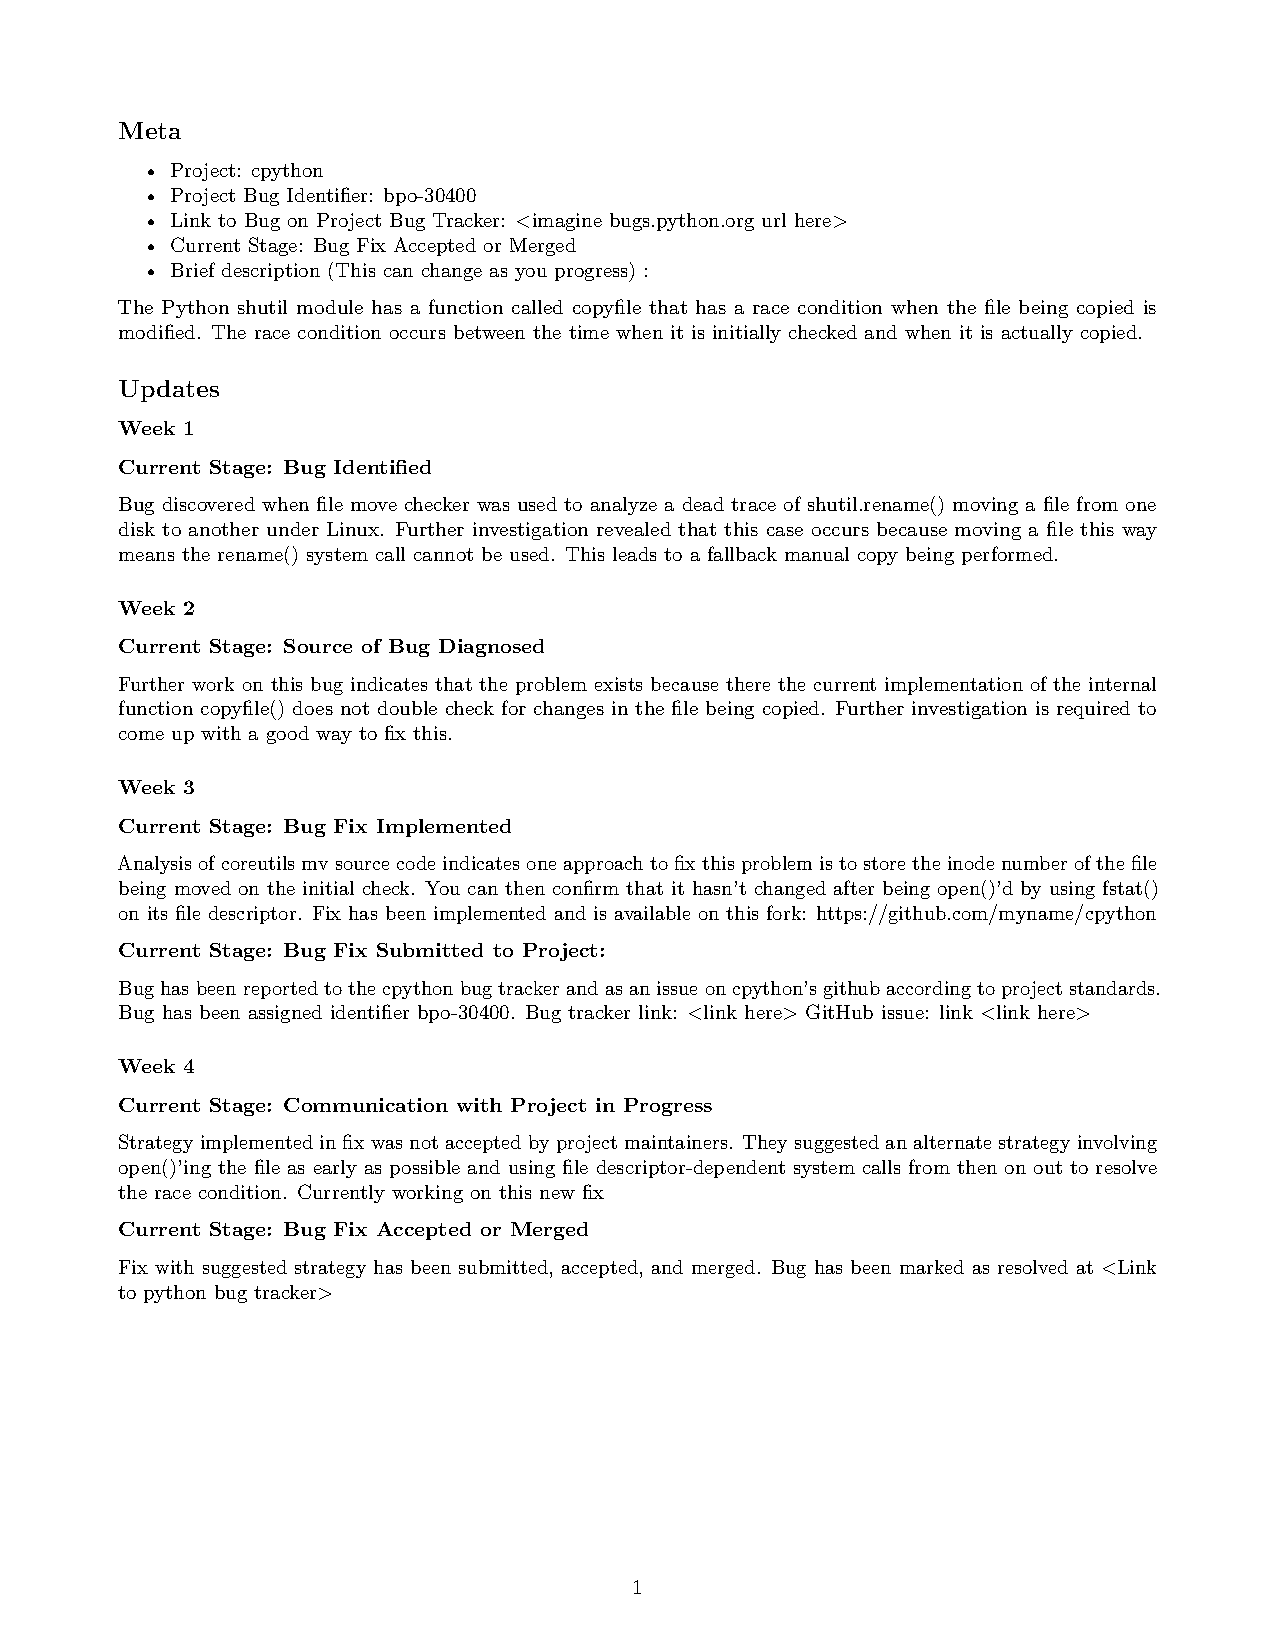
\includegraphics[scale=.8]{chapter4/figures/examplereport}}
\caption[Example Progress Report]{Example Progress Report}
\label{fig:examplereport}
\end{figure}
\restoregeometry

\subsection{Bugs Found by Participants}
\label{subsec:bugs-by-participants}
Study participants using CrashSimulator found a total of 18 bugs
using the ``Unusual Filetype Mutator.''
Students constructed patches to correct six of these bugs and submitted
them to the appropriate maintainers.
Two of the bugs found in the user study
had been previously identified
in our evaluation.
The overlapping bugs were found independently,
as the students weren't aware of the paper or the evaluation results.
To make sure our total counts were not inflated,
we decided to count evaluation bugs and user study bugs separately.
As a result, the tables and counts in earlier
sections do not reflect these 18 bugs.

These results are important
because they confirm
users other than the original development team
can use the tool to find bugs in real world applications.
Participants commented that narrowing the source of a bug
down to a particular sequence of system calls
was helpful in identifying the area of
code responsible for the bug -- a feature
that decreased the time required to produce a fix.
Though observation of study participants
showed that familiarity with operating systems concepts
made it easier to work with CrashSimulator,
those without this background were still able to identify bugs using the
built-in anomalies.




 \begin{figure}
 \begin{lstlisting}[basicstyle=\ttfamily,gobble=4]
     --- ./coreutils_original/coreutils-8.28/src/uniq.c
     +++ ./src/uniq.c
     @@ -333,6 +333,11 @@
      {
        struct linebuffer lb1, lb2;
        struct linebuffer *thisline, *prevline;
     +  struct stat sb;
     +
     +  stat(infile, &sb);
     +  if (S_ISBLK (sb.st_mode) || S_ISCHR (sb.st_mode))
     +    die (EXIT_FAILURE, errno, "error opening device file %s",
              quotef (infile));

        if (! (STREQ (infile, "-") || freopen (infile, "r", stdin)))
          die (EXIT_FAILURE, errno, "%s", quotef (infile));
\end{lstlisting}
\caption[Participant Submitted Patch]{Example of patch submitted by a CrashSimulator user study participant.
This patch prevents the coreutils `uniq` utility from processing block devices. }
\label{fig:participantpatch}
\end{figure}

\subsection{Tool Limitations Identified by Participants}
\label{subsec:crashsim-patches}

As we will explain in more detail in Section~\ref{sec:future-work},
we believe building a community around CrashSimulator is essential to its
continued development and adoption.  Our user study confirmed this belief.
Students submitted five patches
to the tool's code over the
course of the study period.
Three of these reports included patches built by the reporting student that
correct the bug.
The remaining two patches fixed issues with the
Dockerfile used to build a container with CrashSimulator installed.

The students also submitted 33 reports pertaining to problems in CrashSimulator.
Of these, 16 specifically requested support for a new system call that
CrashSimulator had not handled before.  The remaining 17 reported bugs in
existing system call handlers or test orchestration code.
On the one hand this is encouraging.  The necessity of adding
support for new system calls
indicates that the students were
using CrashSimulator to test a wide variety of new applications.
On the other hand, the number of bug reports not related to system call support
indicates there is still work to be done on the tool.
It is our goal that progress on both of these fronts will be driven by
CrashSimulator's community.

\subsection{Tool Shortcomings Identified by Observation of Participants}
\label{subsec:tool-shortcomings}
Observations of the students as they used the tool were also revealing.
First,
it became clear that the tool
lacks a dedicated mechanism
for determining
which application behaviors constitute a ``bug.''
For example, an application's developer
may have intended that an application processing an ``infinitely long'' file should run continuously
until killed by an outside command.
Therefore, that behavior should not be classified as a bug.
Second,
it demonstrated that
simply reporting that an application did or did not change its behavior
in the presence of an anomaly may not provide sufficient data to identify a bug. The results indicating the presence of a bug must be clear to the user.
Both of these issues are being corrected
by improving the tool's outputs.
By more clearly describing
the nature of a given result,
users can have a better idea
if,
and why,
they should be concerned.

To conclude, our user study has revealed both strengths and weakness
with the CrashSimulator tool.  Section~\ref{sec:future-work}
discusses our plans to improve
these weak areas and capitalize on the tool's strengths.
